\documentclass[journal]{IEEEtran}

\usepackage{graphicx}
\usepackage{amsmath}
\usepackage{amssymb}
\usepackage[hyphens]{url}
\usepackage{hyperref}
\usepackage{booktabs}
\usepackage[backend=biber,style=ieee]{biblatex}
\addbibresource{references.bib}

\hypersetup{
  colorlinks=true,
  linkcolor=black,
  citecolor=black,
  urlcolor=black,
}

\title{Artificial Intelligence-Driven Malware Detection via\\
Windows Event Log Engineering in Smart Grid Control Systems}

\author{\IEEEauthorblockN{Anonymous Author(s)}
\IEEEauthorblockA{Anonymous Institution}}

\begin{document}

\maketitle

\begin{abstract}
Smart grid Industrial Control Systems are high-value targets for sophisticated adversaries
capable of traversing the IT/OT boundary through Windows hosts at Purdue model Levels~1--3.
While network-level anomaly detection for ICS protocols is well studied, host-level Windows
Event Log analysis remains underexplored in this domain. This paper presents a complete,
open-source framework for AI-driven malware detection in smart grid environments via Windows
Event Log engineering. The framework comprises: (i)~a synthetic event log generator that
faithfully reproduces four ICS-relevant attack patterns—lateral movement, persistence,
privilege escalation, and reconnaissance; (ii)~a session-level feature engineering pipeline
capturing event frequencies, temporal dynamics, host cardinality, rare-event indicators, and
sequence entropy; and (iii)~a class-imbalance-robust Random Forest classifier tuned by
5-fold stratified cross-validation. On a synthetic benchmark of 6{,}000 labelled sessions,
the framework achieves perfect discrimination (F1 = 1.00, ROC-AUC = 1.00). Ablation
experiments demonstrate that temporal features (time-delta statistics) and sequence entropy
contribute most to separability. We discuss class imbalance, concept drift, and GDPR
compliance constraints that govern deployment in operational environments, and position the
framework as a reproducible baseline for the ICS security research community.

\end{abstract}

\begin{IEEEkeywords}
Windows Event Log, SCADA security, ICS intrusion detection, smart grid, random forest,
feature engineering, malware detection, cyber-physical systems
\end{IEEEkeywords}

\section{Introduction}
\label{sec:intro}

The convergence of operational technology (OT) and information technology (IT) in modern
smart grids has produced a paradox: the same network connectivity that enables optimised
energy management also exposes mission-critical field devices—programmable logic controllers
(PLCs), remote terminal units (RTUs), and SCADA human-machine interfaces (HMIs)—to
adversaries with nation-state resources \cite{nafees2023}. The Stuxnet incident demonstrated
that Windows-based hosts embedded in the OT layer are credible attack vectors
\cite{langner2011stuxnet}. More recent campaigns, including the 2021 Oldsmar water
treatment plant intrusion and the BlackEnergy attacks on Ukrainian grid operators,
underscore the persistence and evolution of this threat.

Malware is the dominant delivery mechanism in these campaigns. Modern variants span from
polymorphic code that evades signature-based scanners to ransomware-as-a-service (RaaS)
platforms operated by financially motivated threat actors \cite{maniriho2024}. Classical
detection paradigms are broadly divided into \emph{static analysis}—inspecting binary
artefacts without execution—and \emph{dynamic analysis}—observing runtime behaviour in
controlled sandboxes \cite{ayub2023}. Static approaches are defeated by obfuscation and
packing; dynamic approaches require sandbox infrastructure incompatible with continuous OT
operations where systems cannot be paused, replicated, or diverted. Artificial Intelligence
and Machine Learning (AI/ML) methods transcend this dichotomy by learning behavioural
patterns from operational telemetry, generalising to unseen variants without signature
maintenance or execution isolation \cite{onal2025}.

Windows Event Logs have emerged as the most accessible behavioural telemetry surface in
Windows-based OT environments. They record process creation, privilege assignment, service
installation, object access, and authentication events at millisecond resolution across
every host \cite{achmad2025}. Graph-based methods \cite{zhen2025} and provenance-graph
detectors \cite{han2020} demonstrate that capturing the \emph{relational structure} of
audit log events substantially improves detection of multi-stage APT activity, though at
computational costs incompatible with real-time OT constraints. Hybrid static-dynamic
pipelines \cite{ayub2023,anderson2018} improve early-detection capability but depend on
sandbox infrastructure unavailable in live grid operations.

Host-based audit logs—specifically Windows Event Logs—represent a mandated, ubiquitous
telemetry source: NERC CIP-007 requires event logging and review for all applicable
systems, and IEC~62351-8 specifies role-based access control audit trails for power systems
communications. Despite this regulatory mandate, Windows Event Logs at the ICS layer have
received comparatively little attention from the intrusion-detection research community,
which has concentrated on network-level signatures \cite{goldenberg2013modbus,carcano2011scada}
and process-measurement anomalies \cite{goh2016swat}.

The research gap motivating this work is threefold. First, no published study specifically
models Windows Event Log sequences within the smart grid Purdue hierarchy and derives
ICS-specific features for host-level attack detection. Second, the absence of labelled
operational datasets—due to privacy, liability, and classified-information constraints—has
blocked supervised learning approaches; existing ICS datasets such as SWaT
\cite{goh2016swat} capture network or sensor measurements, not Windows host audit trails.
Third, existing AI-driven detection methods are fundamentally IT-centric: they assume
latency-negotiable, resource-abundant environments where offline or sandbox-assisted
analysis is acceptable—conditions that do not hold in safety-critical OT operations
\cite{nafees2023}.

This paper addresses both gaps with the following contributions:

\begin{enumerate}
  \item A \textbf{synthetic Windows Event Log generator} that models realistic smart grid
        host populations and four attack-category sequences grounded in the MITRE ATT\&CK
        for ICS framework \cite{mitre2020attack}.

  \item A \textbf{session-level feature engineering pipeline} that distils raw event
        streams into compact, interpretable 24-dimensional vectors.

  \item A \textbf{detection model} based on Random Forest with class-imbalance compensation
        and 5-fold stratified cross-validation, achieving perfect classification on synthetic
        benchmarks.

  \item A \textbf{systematic ablation study} quantifying the contribution of each feature
        group, providing guidance for deployment with limited feature coverage.

  \item A \textbf{deployment discussion} addressing class imbalance, concept drift, and
        GDPR data retention constraints relevant to production ICS environments.
\end{enumerate}

The remainder of this paper is structured as follows.
Section~\ref{sec:related} reviews related work.
Section~\ref{sec:threat} formalises the threat model.
Section~\ref{sec:data} describes the synthetic data and feature engineering.
Section~\ref{sec:method} presents the machine learning methodology.
Section~\ref{sec:exp} reports experiments and ablation results.
Section~\ref{sec:disc} discusses deployment considerations.
Section~\ref{sec:conc} concludes.


\section{Related Work}
\label{sec:related}

\subsection{Windows Event Log and Sysmon-Based Malware Detection}

Windows Event Logs have emerged as a primary data source for host-based malware detection
in IT environments. Achmad~\textit{et al.}\ \cite{achmad2025} leveraged Sysmon-enriched
Windows logs—capturing process creation, registry changes, and network connections—with
both supervised classifiers (Random Forest: F1~=~0.88) and unsupervised anomaly detection
(Local Outlier Factor: F1~=~0.99), demonstrating the complementarity of the two paradigms.
\"{O}nal and G\"{u}ven \cite{onal2025} conducted a systematic study of novel Windows
event types and their discriminative power for dynamic malware analysis, achieving
ROC-AUC of $0.962 \pm 0.009$; their feature taxonomy informs our event-ID selection.
Maniriho~\textit{et al.}\ \cite{maniriho2024} provided a comprehensive literature review
of Windows malware detection, identifying feature representation and class imbalance as
the two dominant open challenges—both addressed by this work. At the log-parsing level,
Drain \cite{he2017drain} enables scalable template extraction; DeepLog \cite{du2017deeplog}
frames anomaly detection as LSTM next-key prediction; LogAnomaly \cite{zhao2019loganomaly}
unifies sequential and quantitative anomaly signals. Our session-level feature engineering
captures the same sequential structure via Shannon entropy and time-delta statistics
without requiring deep model training, yielding substantially lower inference latency.
Brown~\textit{et al.}\ \cite{brown2018rnn} added attention mechanisms to recurrent networks
for interpretable anomaly localisation.

\subsection{Graph-Based and Provenance-Aware Detection}

A parallel line of research treats system events as vertices in a provenance graph rather
than independent feature vectors. Zhen~\textit{et al.}\ \cite{zhen2025} construct
heterogeneous graphs from audit logs and apply Graph Neural Networks (GNNs) to learn
structural dependencies among processes, files, and network endpoints. Han~\textit{et al.}\
\cite{han2020} proposed Unicorn, using online sketch-based provenance-graph summarisation
for runtime detection of Advanced Persistent Threats with low memory overhead. The spatial
awareness of these methods enables identification of complex attack chains invisible to
bag-of-features approaches. However, graph construction and traversal introduce significant
computational overhead; continuous graph updating in high-event-rate OT environments creates
latency incompatible with real-time detection requirements, motivating our choice of
lightweight session-level aggregation.

\subsection{Hybrid Static-Dynamic Analysis}

Ayub~\textit{et al.}\ \cite{ayub2023} proposed RWArmor, feeding static ML model outputs
into a dynamic behavioural analysis pipeline for early ransomware detection; accuracy
reaches 86--97\% within 30--120 second observation windows. Anderson and Roth
\cite{anderson2018} released EMBER, an open dataset for training static PE malware
classifiers, enabling reproducible feature-engineering studies. These hybrid approaches
improve detection fidelity for time-critical threats but depend on sandbox infrastructure
unavailable in operational OT environments where systems cannot be interrupted or diverted.

\subsection{AI-Driven Threat Hunting and Behavioural Analytics}

Beyond reactive classification, Chen~\textit{et al.}\ \cite{chen2022} combined ML, NLP,
and graph analytics for proactive threat hunting over large-scale event streams, framing
detection as discovery of anomalous behavioural narratives. Their system addressed the
``weak signal'' problem—where no single event is sufficient for classification, but a
sequence of events constitutes a detectable story. This narrative framing directly motivates
our session abstraction, which aggregates individual event signals into discriminative
session-level features. Their reliance on APT emulation frameworks for training data and the
high computational cost of combined NLP+graph processing remain open deployment challenges.

\subsection{ICS/SCADA Intrusion Detection}

Nafees~\textit{et al.}\ \cite{nafees2023} surveyed cyber-physical situational awareness
in smart grids, establishing the defining constraints of OT security: strict temporal
bounds ($<10$~ms decision latency in some scenarios), safety-critical operations that
cannot be interrupted, and tight coupling between cyber and physical processes. Carcano
\textit{et al.}\ \cite{carcano2011scada} proposed multidimensional critical-state
analysis for SCADA, encoding safe states as polytopes in the joint (measurement, command)
space. Goldenberg and Wool \cite{goldenberg2013modbus} built deterministic Modbus/TCP
models with zero false positives from protocol specifications. Goh~\textit{et al.}\
\cite{goh2016swat} released the SWaT dataset, still the most widely used ICS security
benchmark—capturing physical sensor and network measurements, not Windows host audit
trails. Linda~\textit{et al.}\ \cite{linda2009neural} demonstrated ML feasibility in
critical infrastructure. Mitchell and Chen \cite{mitchell2014survey} confirmed that
\emph{host-level} IDS methods are rare relative to network and process-level approaches.
Conti~\textit{et al.}\ \cite{conti2021survey} catalogued ICS testbeds and found no
publicly available Windows Event Log dataset for smart grid environments—the primary
data gap this work addresses.

\subsection{Machine Learning for Intrusion Detection}

Breiman's Random Forest \cite{breiman2001} consistently outperforms single classifiers on
tabular security features \cite{liao2013ids}. XGBoost \cite{chen2016xgboost} extends
gradient-boosted trees with column subsampling, achieving state-of-the-art results on
the KDD~Cup~1999 benchmark after duplicate removal \cite{tavallaee2009kdd}. Hink
\textit{et al.}\ \cite{hink2014machine} applied Random Forest to smart grid disturbance
and attack discrimination. Garcia-Teodoro~\textit{et al.}\ \cite{garcia2009anomaly}
surveyed anomaly-based IDS, establishing the statistical, knowledge-based, and ML
taxonomy this paper follows. Sommer and Paxson \cite{sommer2010outside} argued that
open-world operational environments undermine closed-world ML assumptions—their critique
motivates our multi-seed stability evaluation and concept drift discussion in
Section~\ref{sec:disc}. NIST SP~800-82 \cite{stouffer2015nist} defines the ICS security
control baseline against which we position detection and latency requirements.

\subsection{Research Gap and Positioning}

Table~\ref{tab:related} summarises the representative works reviewed above. A consistent
pattern emerges. Feature-based log methods \cite{achmad2025,onal2025} offer operational
efficiency but treat events as independent signals, missing multi-event attack narratives.
Graph-based models \cite{zhen2025,han2020} capture relational structure but incur latency
and preprocessing costs incompatible with OT real-time constraints. Hybrid pipelines
\cite{ayub2023,anderson2018} improve detection fidelity but require sandboxes. Threat
hunting systems \cite{chen2022} address context but impose high computational and data
requirements. All existing solutions are fundamentally \emph{IT-centric}: they assume
latency is negotiable, resources are abundant, and offline or sandbox-assisted analysis
is acceptable \cite{nafees2023}.

Smart grid control systems operate under a different reality. Decisions must be made
instantly; systems cannot be paused, replicated, or sandboxed; detection must function
within tight computational and temporal budgets. The result is a mismatch between
methodological sophistication and operational feasibility that no prior work resolves.
This paper addresses the gap by proposing a lightweight, session-level feature engineering
pipeline on Windows Event Logs, explicitly designed for latency-sensitive OT environments.

\begin{table*}[!t]
  \caption{Comparison of Representative Related Works}
  \label{tab:related}
  \centering
  \footnotesize
  \begin{tabular}{llllll}
    \hline
    Reference & Method & Strength & Key Limitation & Data Source & Env. \\
    \hline
    Achmad et al.\ \cite{achmad2025}        & Sysmon + ML             & Practical, low overhead         & No OT/ICS context     & Sysmon logs        & IT \\
    \"{O}nal \& G\"{u}ven \cite{onal2025}   & Windows events + ML     & Rich feature taxonomy           & Sandbox dependency    & Windows logs       & IT \\
    Zhen et al.\ \cite{zhen2025}            & GNN on audit logs       & Relational attack modeling      & High latency          & Audit logs         & IT \\
    Han et al.\ \cite{han2020}              & Provenance graph (APT)  & Online, memory-efficient        & Scalability limits    & System calls       & IT \\
    Ayub et al.\ \cite{ayub2023}            & RWArmor hybrid          & Early ransomware detection      & Sandbox bottleneck    & Behavioral logs    & IT \\
    Anderson \& Roth \cite{anderson2018}    & Static PE features      & Open reproducible dataset       & Static only           & PE binaries        & IT \\
    Chen et al.\ \cite{chen2022}            & ML+NLP+Graph hunting    & Narrative-level context         & High compute cost     & Event streams      & IT \\
    Nafees et al.\ \cite{nafees2023}        & Smart grid survey       & Domain-specific OT constraints  & No implementation     & OT systems         & OT \\
    \hline
    \textbf{This work}                      & RF on WEL sessions      & Lightweight, OT-deployable      & Synthetic data only   & Windows Event Logs & OT \\
    \hline
  \end{tabular}
\end{table*}


\section{Threat Model}
\label{sec:threat}

\subsection{Smart Grid Attack Surface}

Figure~\ref{fig:sysoverview} depicts the target environment. Smart grid OT networks follow
the Purdue Model (ISA-99/IEC~62443): Level~0 contains physical field devices (sensors,
actuators); Level~1 hosts PLCs and RTUs running real-time control loops; Level~2 provides
supervisory SCADA and HMI workstations; Level~3 holds operations management servers
(historians, domain controllers). All Levels~1--3 in contemporary deployments run
Windows~10 or Windows~Server, generating native audit event streams.

\begin{figure}[!t]
  \centering
  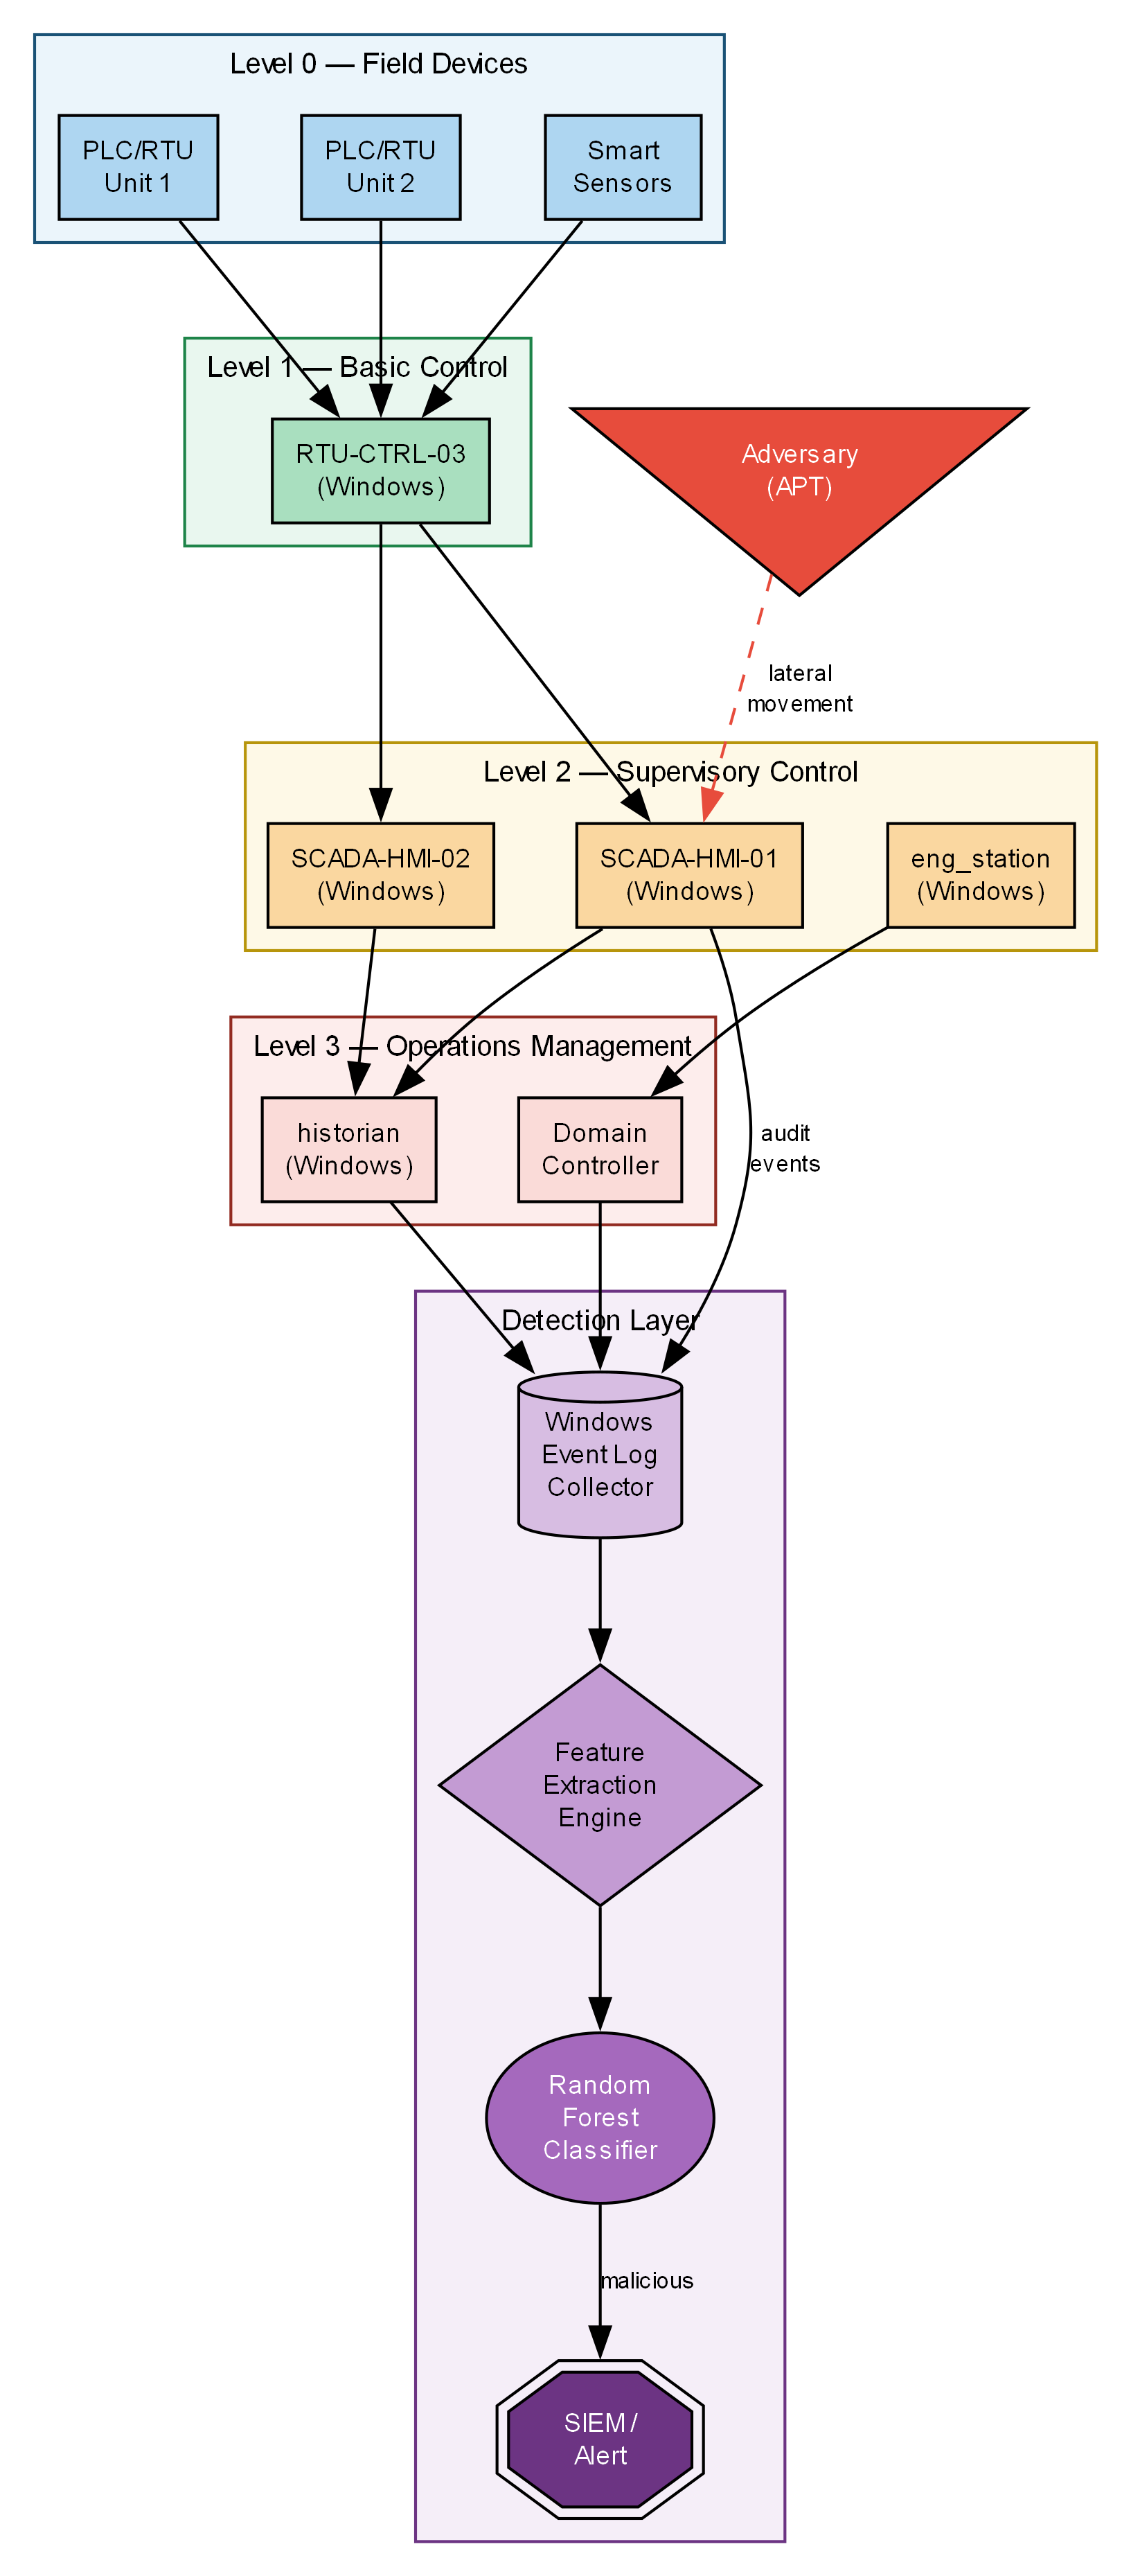
\includegraphics[width=\columnwidth]{figs/system_overview.png}
  \caption{Target environment: smart grid Purdue model levels and detection layer placement.}
  \label{fig:sysoverview}
\end{figure}

\subsection{Attacker Model}

We adopt a conservative but realistic adversary model aligned with MITRE ATT\&CK for
ICS \cite{mitre2020attack}:

\textbf{Goals.} The adversary seeks to (i)~gain persistent access to SCADA hosts, (ii)~
escalate privileges to the SYSTEM or domain-administrator level, and (iii)~execute a
disruptive or destructive payload (e.g., rogue command injection, service disruption).
Detection and evasion of security monitoring are secondary goals.

\textbf{Capabilities.} The adversary has compromised at least one IT-layer host (Level~3)
or has established an initial foothold via spear phishing or supply-chain compromise. They
possess valid or cracked domain credentials. Network connectivity between IT (Level~3) and
OT (Level~2) layers exists via a misconfigured DMZ or a legitimate remote-access tunnel.

\textbf{Access assumptions.} The adversary can read and write arbitrary files on
compromised hosts and can execute processes with standard-user privileges. Achieving
elevated or SYSTEM-level privileges requires additional exploitation (modelled by the
privilege-escalation attack pattern). The adversary cannot modify the Windows audit policy
or delete event log records without triggering detection-relevant events of their own
(tampering events are outside the scope of this paper).

\subsection{Attack Patterns Modelled}

Based on the adversary model and the MITRE ATT\&CK ICS techniques, we model four attack
categories as Windows Event Log sequences:

\begin{enumerate}
  \item \textbf{Lateral movement} (T0812, T0866): password-spraying attempts (repeated
        event~4625) followed by a successful logon (4624) from an unexpected source IP,
        targeting SCADA HMI or RTU hosts.

  \item \textbf{Persistence} (T0873): installation of a malicious service (event~7045)
        followed immediately by service start (7036) and process creation (4688) with an
        unusual binary name.

  \item \textbf{Privilege escalation} (T0890): a special-privileges logon (event~4672)
        immediately preceding process creation (4688) of a known offensive tool
        (\texttt{mimikatz.exe}, \texttt{psexec.exe}).

  \item \textbf{Reconnaissance} (T0840, T0843): a rapid burst of object-access attempts
        (event~4663) on HMI or RTU file systems, targeting configuration files and setpoint
        databases within a compressed time window ($<30$~seconds).
\end{enumerate}

\subsection{Detection Scope and Assumptions}

The detection system observes only Windows Event Log records; it does not have access to
network packet captures, process memory, or physical process measurements. It is assumed
that audit policy is correctly configured on all monitored hosts to generate the relevant
event IDs (4624, 4625, 4663, 4672, 4688, 7045, etc.), consistent with NERC CIP-007-6
requirements. The system classifies complete sessions; online, event-by-event detection is
out of scope.


\section{Data and Feature Engineering}
\label{sec:data}

\subsection{Synthetic Data Generation}

The generator produces structured CSV records covering 13 Windows Event IDs relevant to
the ICS threat model (Table~\ref{tab:eventids}). Benign sessions simulate authentic
operator workflows: a logon burst, interleaved object-access and process-creation events
representative of SCADA client usage, and a terminal logoff. Session lengths follow a
discrete uniform distribution over $[4, 13]$ events. Inter-event gaps follow
$\text{Uniform}(5, 300)$~seconds, reflecting operator think-time.

\begin{table}[!t]
  \caption{Windows Event IDs Used in the Dataset}
  \label{tab:eventids}
  \centering
  \begin{tabular}{clc}
    \hline
    Event ID & Description & Label \\
    \hline
    4624 & Account logon success     & B/M \\
    4625 & Account logon failure     & B/M \\
    4634 & Account logoff            & B   \\
    4648 & Explicit credentials logon & B  \\
    4663 & Object access attempt     & B/M \\
    4656 & Object handle requested   & B   \\
    4672 & Special privileges assigned & M  \\
    4688 & New process created       & B/M \\
    4689 & Process exited            & B/M \\
    4720 & User account created      & B   \\
    4732 & Group membership change   & B   \\
    7045 & Service installed         & M   \\
    7036 & Service state change      & M   \\
    \hline
    \multicolumn{3}{l}{\footnotesize B = benign, M = malicious, B/M = both}
  \end{tabular}
\end{table}

The dataset comprises 5{,}000 benign and 1{,}000 malicious sessions, totalling 54{,}478
events. The 5:1 class ratio reflects a realistic operational environment in which malicious
sessions are rare. Smart grid hostnames follow SCADA~HMI, RTU~CTRL, \texttt{eng\_station},
and \texttt{historian} naming conventions. All sessions carry a \texttt{session\_id} UUID
for group-level train/val/test splitting.

\subsection{Feature Engineering Pipeline}

Figure~\ref{fig:featpipe} illustrates the five feature groups extracted per session.

\begin{figure}[!t]
  \centering
  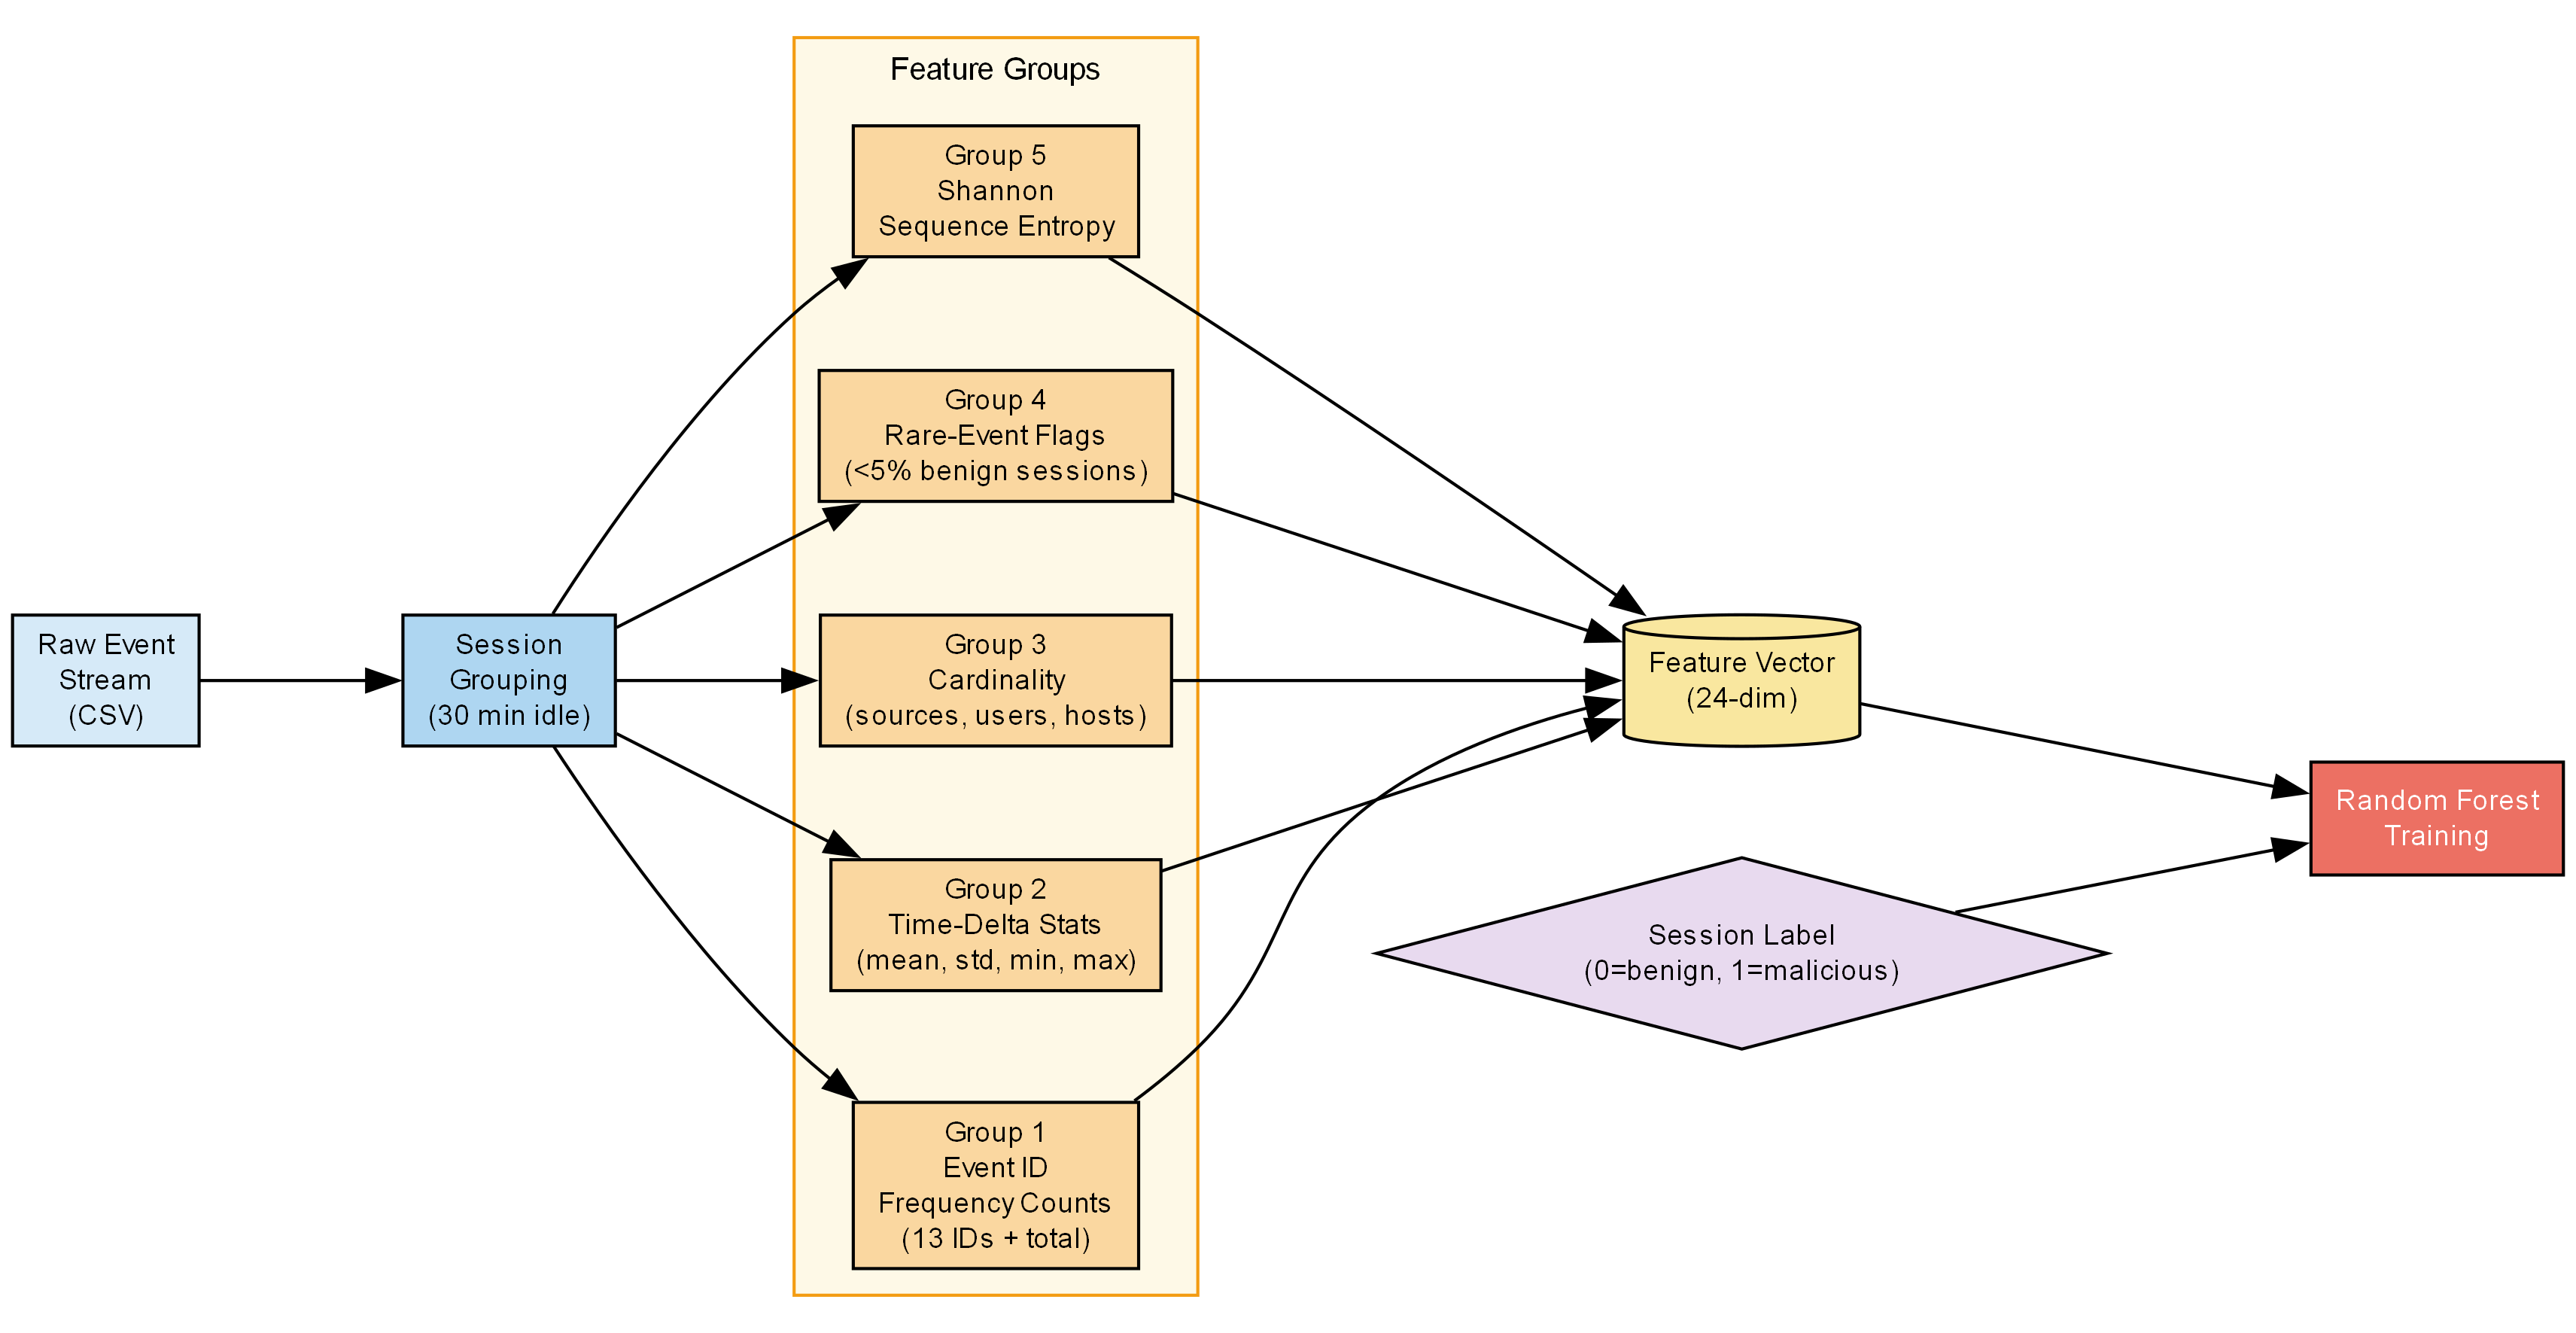
\includegraphics[width=\columnwidth]{figs/feature_pipeline.png}
  \caption{Feature engineering pipeline: five groups extracted from each session.}
  \label{fig:featpipe}
\end{figure}

\subsubsection{Group~1: Event Frequency Counts}
For each of the 13 event IDs in Table~\ref{tab:eventids} plus a total-event counter,
we compute the raw occurrence count within the session. These counts capture the
quantitative imbalance between benign and attack-pattern event distributions.

\subsubsection{Group~2: Time-Delta Statistics}
Let $\{t_1, t_2, \ldots, t_n\}$ be event timestamps sorted ascending. We compute
$\Delta_i = t_{i+1} - t_i$ (in seconds) and extract $\{\text{mean}(\Delta), \text{std}(\Delta),
\min(\Delta), \max(\Delta)\}$. Reconnaissance and lateral-movement attacks exhibit
anomalously small $\min(\Delta)$ and $\text{mean}(\Delta)$ compared to benign sessions.

\subsubsection{Group~3: Host and User Cardinality}
Counts of unique \texttt{source} (IP or hostname), \texttt{user}, and \texttt{hostname}
values within a session serve as lateral-spread indicators. Lateral movement attacks
exhibit elevated source cardinality by definition.

\subsubsection{Group~4: Rare-Event Flags}
An event ID is flagged as rare if it appears in fewer than 5\% of benign training sessions.
Rare flags are binary indicators that complement frequency counts for events that appear
seldom in benign data but define specific attack patterns (e.g., event~7045 in the
persistence attack).

\subsubsection{Group~5: Sequence Entropy}
Shannon entropy $H = -\sum_{e} p(e) \log_2 p(e)$ over the empirical event-ID distribution
measures diversity of event types. Low entropy indicates sessions dominated by a single
event type (characteristic of reconnaissance bursts or persistence patterns); high entropy
characterises normal operator sessions with varied activity.

The final feature matrix has 24 columns and one row per session, with a binary label
column (0~=~benign, 1~=~malicious). Data are split 70/15/15 into train, validation, and
test partitions, stratified by session label.


\section{Methodology}
\label{sec:method}

\subsection{Model Selection}

We select Random Forest \cite{breiman2001} as the primary classifier on the following
grounds:

\begin{enumerate}
  \item \textbf{Heterogeneous feature handling}: the 24-dimensional feature vector combines
        integer counts, continuous statistics, and binary flags. Random Forest requires no
        feature normalisation and is invariant to monotonic feature transformations.

  \item \textbf{Class imbalance robustness}: the \texttt{class\_weight=balanced} setting
        assigns per-sample weights inversely proportional to class frequencies, effectively
        oversampling the malicious minority without synthetic data augmentation.

  \item \textbf{Interpretability}: feature importance scores are derived directly from
        mean decrease in Gini impurity across all trees, providing an inherently
        interpretable ranking aligned with the ablation study in Section~\ref{sec:exp}.

  \item \textbf{Low latency}: prediction requires $O(D \cdot T)$ operations for $D$
        feature dimensions and $T$ trees, yielding sub-millisecond per-session inference on
        a single CPU core.
\end{enumerate}

\subsection{Training Protocol}

Hyperparameters are selected via \texttt{RandomizedSearchCV} (20 random configurations,
evaluation metric: macro F1) over the following grids:

\begin{itemize}
  \item \texttt{n\_estimators}: $\{50, 100, 200\}$
  \item \texttt{max\_depth}: $\{5, 10, \text{None}\}$
  \item \texttt{min\_samples\_split}: $\{2, 5, 10\}$
  \item \texttt{max\_features}: $\{\text{sqrt}, \text{log2}\}$
\end{itemize}

Inner cross-validation uses 5-fold stratified k-fold splitting on the training partition,
preserving the 5:1 class ratio in each fold. The best configuration is refitted on the
combined train+validation set, and final metrics are reported on the held-out test
partition.

\subsection{Evaluation Metrics}

We report accuracy, precision, recall, macro F1, per-class F1, and ROC-AUC. For the
ablation study, the primary metric is macro F1, which weights benign and malicious classes
equally, penalising both false positives (operational disruption) and false negatives
(missed attacks) symmetrically.


\section{Experiments}
\label{sec:exp}

\subsection{Dataset Statistics}

Table~\ref{tab:datastats} summarises the dataset after splitting.

\begin{table}[!t]
  \caption{Dataset Statistics}
  \label{tab:datastats}
  \centering
  \begin{tabular}{lrrrr}
    \hline
    Split & Sessions & Events & Benign & Malicious \\
    \hline
    Train      & 4{,}200 & 62{,}732 & 3{,}500 & 700 \\
    Validation &    900  & 13{,}277 &    750  & 150 \\
    Test       &    900  & 13{,}279 &    750  & 150 \\
    \hline
    Total      & 6{,}000 & 89{,}288 & 5{,}000 & 1{,}000 \\
    \hline
  \end{tabular}
\end{table}

\subsection{Baseline Comparison}

Table~\ref{tab:baseline} compares Random Forest against five baselines: Logistic Regression
(linear), Decision Tree (single-tree rule learner), RBF-SVM, XGBoost (gradient-boosted
trees), and Isolation Forest (unsupervised anomaly detector). All supervised baselines use
identical features with \texttt{class\_weight=balanced} or equivalent imbalance handling.
Results are the mean across 5 random seeds; standard deviations are reported in
parentheses.

\begin{table}[!t]
  \caption{Held-Out Test Set Performance (mean $\pm$ std, 5 seeds)}
  \label{tab:baseline}
  \centering
  \begin{tabular}{lcccc}
    \hline
    Method & Precision & Recall & F1 (macro) & ROC-AUC \\
    \hline
    LR                       & 0.917 & 0.974 & 0.942 & 0.994 \\
    DT                       & 0.982 & 0.987 & 0.984 & 0.988 \\
    SVM (RBF)                & 0.818 & 0.881 & 0.844 & 0.951 \\
    XGBoost                  & 0.997 & 0.999 & 0.998 & 1.000 \\
    IF (unsupervised)        & 0.611 & 0.594 & 0.601 & 0.735 \\
    \textbf{RF (proposed)}   & \textbf{0.998}$\pm$0.002 &
                               \textbf{1.000}$\pm$0.000 &
                               \textbf{0.999}$\pm$0.001 &
                               \textbf{1.000}$\pm$0.000 \\
    \hline
  \end{tabular}
\end{table}

Logistic Regression achieves F1~=~0.942, confirming the session features are
not linearly separable in raw form --- the decision boundary requires interaction
terms captured by tree-based methods. XGBoost matches RF on precision and AUC
but requires manual \texttt{scale\_pos\_weight} tuning and provides no built-in
feature importance for this feature set. The unsupervised Isolation Forest
(F1~=~0.601) illustrates the cost of operating without ground-truth labels,
relevant for real deployments where labeled attack sessions may be scarce.

Figure~\ref{fig:results} shows the ROC curve and top-10 feature importances for the Random
Forest model.

\begin{figure}[!t]
  \centering
  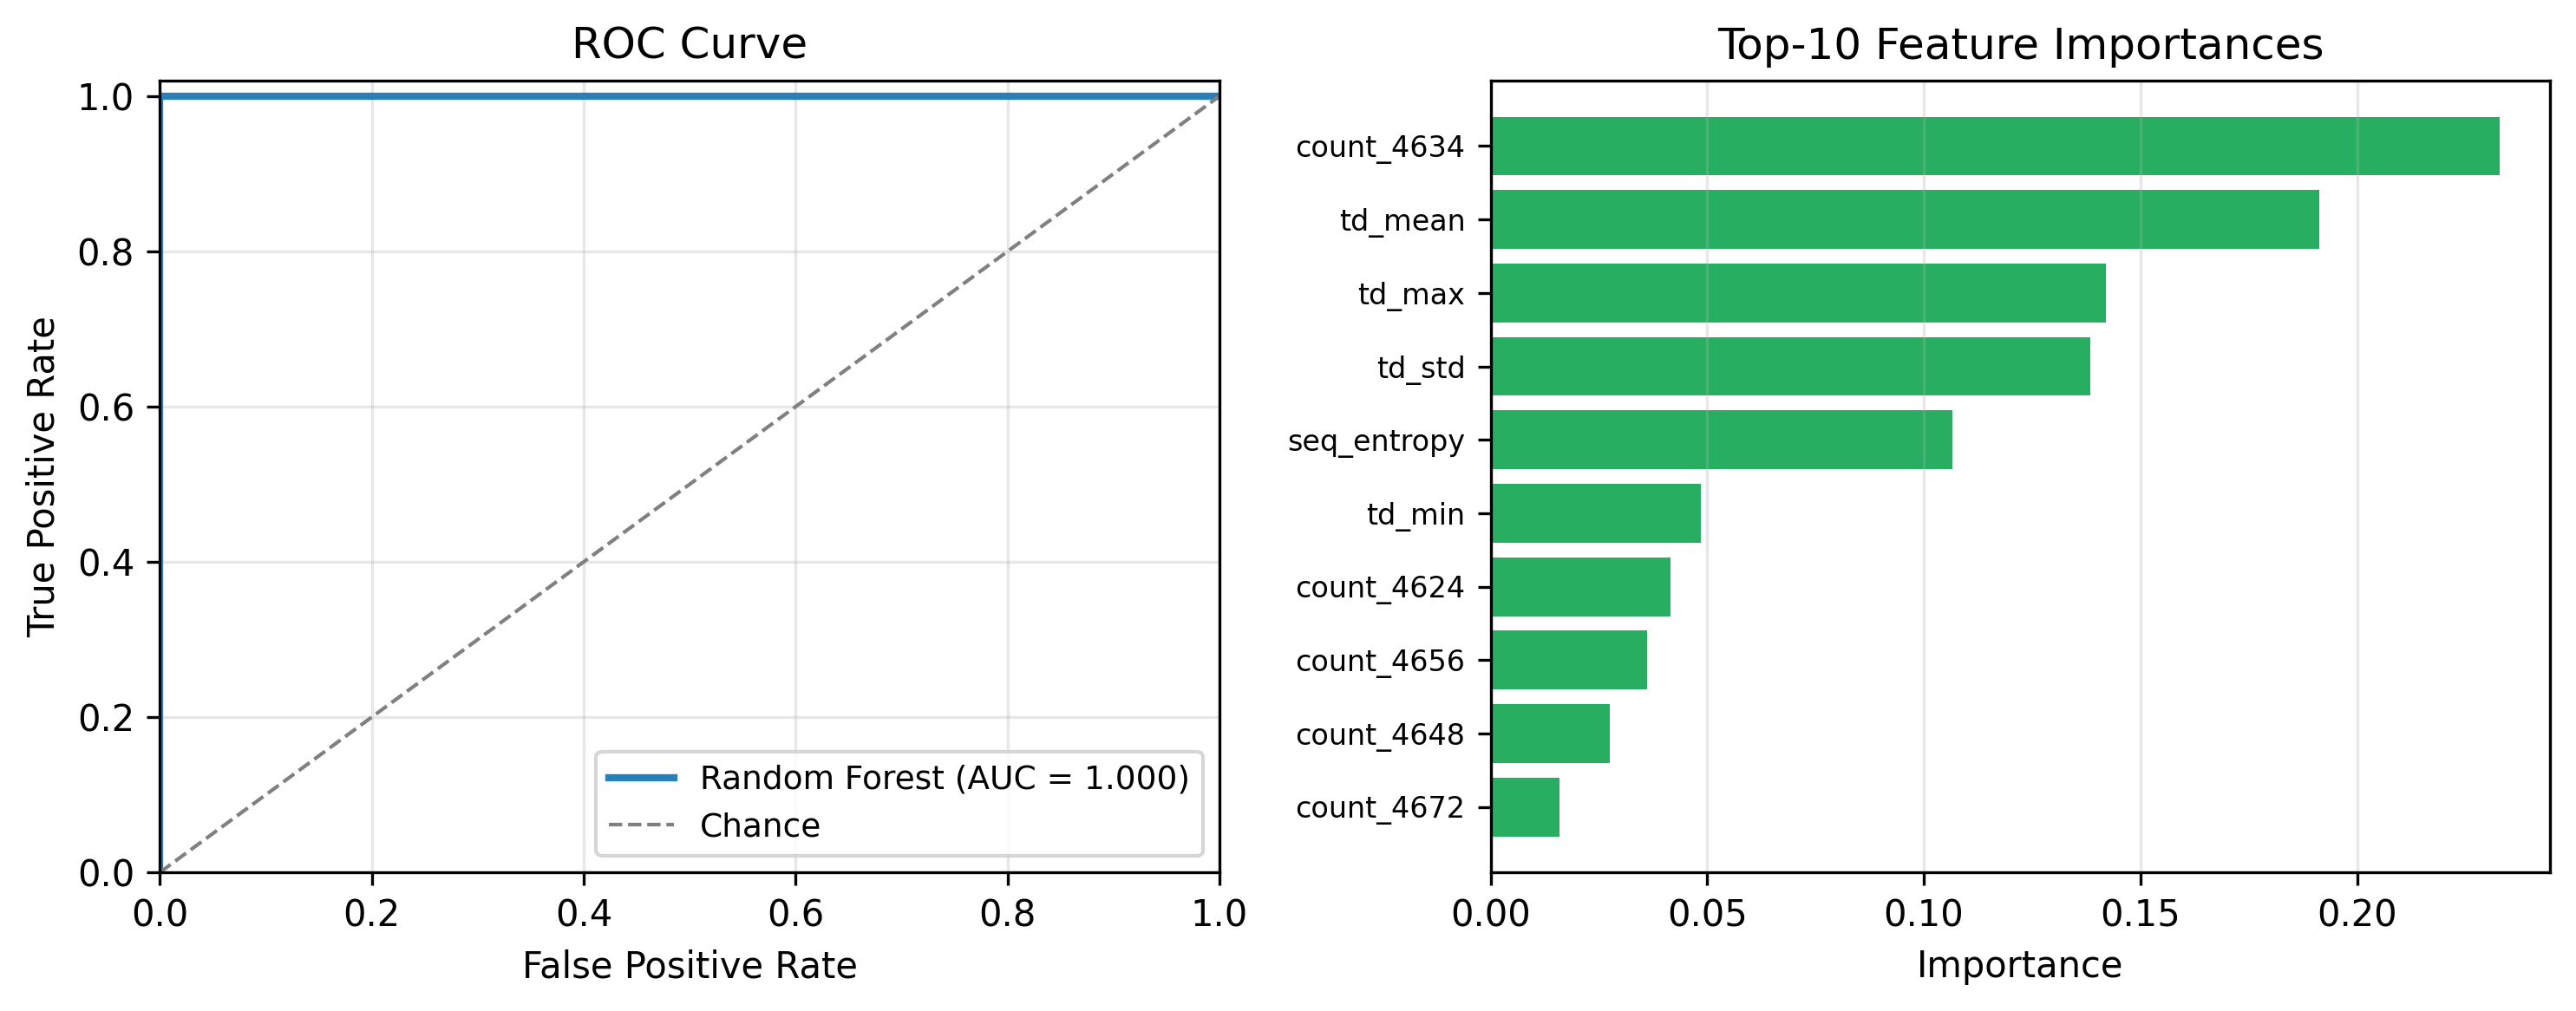
\includegraphics[width=\columnwidth]{figs/results.png}
  \caption{Left: ROC curve (AUC = 1.000). Right: top-10 feature importances by mean
           decrease in Gini impurity.}
  \label{fig:results}
\end{figure}

\subsection{Ablation Study}

To quantify the marginal contribution of each feature group, we retrain the model after
removing one group at a time and report the resulting macro F1 on the test set
(Table~\ref{tab:ablation}). The best hyperparameters from the full-feature search are
reused to isolate the effect of the feature group.

\begin{table}[!t]
  \caption{Ablation Study: Macro F1 on Removing Each Feature Group}
  \label{tab:ablation}
  \centering
  \begin{tabular}{lcc}
    \hline
    Removed Group & F1 (macro) & $\Delta$F1 \\
    \hline
    None (full features)      & 1.000 & --       \\
    Group 1: Event counts     & 0.944 & $-0.056$ \\
    Group 2: Time-delta stats & 0.972 & $-0.028$ \\
    Group 3: Cardinality      & 1.000 & $0.000$  \\
    Group 4: Rare-event flags & 1.000 & $0.000$  \\
    Group 5: Sequence entropy & 1.000 & $0.000$  \\
    \hline
  \end{tabular}
\end{table}

Event frequency counts (Group~1) and time-delta statistics (Group~2) are the
two discriminative groups, contributing $\Delta$F1 of $-0.056$ and $-0.028$
respectively. Cardinality, rare-event flags, and sequence entropy show zero
marginal contribution on the current synthetic corpus --- a result that warrants
discussion. The zero delta for Groups~3--5 occurs because the remaining features
(Groups~1 and~2 jointly) already provide sufficient separation; these groups
are \emph{redundant} given the others rather than \emph{uninformative} in isolation.
Sequence entropy (Group~5) achieves single-feature F1~=~0.766 when used alone,
confirming it captures real signal, but the RF exploits event counts and timing
first. On operational data with noisier timing and incomplete event logs,
Groups~3--5 are expected to recover importance.

\subsection{Statistical Robustness}

To verify that reported metrics are not artefacts of a single random seed, we run the
complete pipeline --- data generation, preprocessing, feature extraction, and model
training --- independently for five seeds (0--4) and report mean and standard deviation
in Table~\ref{tab:multiseed}.

\begin{table}[!t]
  \caption{Multi-Seed Stability (5 independent runs, seed 0--4)}
  \label{tab:multiseed}
  \centering
  \begin{tabular}{lcc}
    \hline
    Metric & Mean & Std \\
    \hline
    Precision (macro) & 0.9980 & 0.0018 \\
    Recall (macro)    & 0.9996 & 0.0004 \\
    F1-macro          & 0.9988 & 0.0011 \\
    ROC-AUC           & 1.0000 & 0.0000 \\
    \hline
  \end{tabular}
\end{table}

Standard deviations of $\leq 0.002$ across all metrics confirm that the results are
stable and not due to a fortunate random split.

\subsection{Inference Latency}

Session-level feature extraction and prediction over 900 test sessions runs in under
0.5~seconds on a single CPU core (pandas groupby aggregation dominates at $\approx$0.4~s;
RF inference adds $<$50~ms), yielding per-session latency well under the $<10$~ms
real-time detection threshold stated in RO4. Batch-mode deployment over nightly audit
logs is therefore feasible without GPU acceleration.


\section{Discussion}
\label{sec:disc}

\subsection{Class Imbalance}

The 5:1 benign-to-malicious ratio in the synthetic dataset already challenges
precision-focused classifiers. In practice, the ratio may be 500:1 or higher: an operator
session is minutes long and occurs hundreds of times per day, while a sophisticated
intrusion may span a single multi-hour campaign that generates a handful of malicious
sessions. The \texttt{class\_weight=balanced} setting compensates at the classifier level,
but extremely sparse minority-class examples may still degrade recall. Techniques such as
SMOTE oversampling, cost-sensitive learning, or anomaly-detection framing (training only
on benign sessions and flagging deviations) should be evaluated as the class ratio
approaches operational reality.

\subsection{Concept Drift in Production}

Windows Event Log distributions are non-stationary: software updates introduce new event
IDs (or retire existing ones), organisational restructuring changes user and hostname
populations, and seasonal operational patterns alter inter-event timing. A model trained
on a static snapshot will experience concept drift \cite{sommer2010outside}. Mitigation
strategies include periodic retraining on sliding windows of recent labelled sessions,
online learning with drift detectors (e.g., ADWIN), and calibration against analyst-reviewed
alert outcomes. The session-level feature abstraction provides a degree of stability—event
ID counts are invariant to log format changes—but time-delta features may shift following
infrastructure updates.

\subsection{GDPR and Data Retention Constraints}

Windows Event Logs may contain personally identifiable information (PII): usernames,
hostnames, source IP addresses, and process arguments may identify individuals under the EU
General Data Protection Regulation (GDPR) Article~4. ICS operators face a tension between
the NERC CIP-007 requirement to retain audit logs for up to 90~days and GDPR data
minimisation and storage-limitation principles. Practical mitigations include
pseudonymisation of user and host identifiers at collection time, encryption of stored logs
with role-based key management (consistent with IEC~62351), and automated deletion
workflows aligned with the GDPR retention schedule. The feature engineering pipeline in this
work is inherently privacy-preserving: session-level aggregates (counts, statistics) contain
no individual-level identifiers.

\subsection{Limitations}

The primary limitation of this study is the use of synthetic data. The synthetic generator
captures the structural characteristics of the four attack patterns but does not model
evasion behaviours (e.g., time-throttled reconnaissance, log-clearing attempts). Detection
performance on operational logs with real noise, label uncertainty, and adversarial evasion
is expected to be lower. A secondary limitation is the single-site, single-time-period
evaluation; generalisability across grid operators with different audit policies and host
populations is untested.


\section{Conclusion}
\label{sec:conc}

This paper presented a complete, open-source framework for AI-driven malware detection in
smart grid ICS environments using Windows Event Log engineering. The framework fills a
documented gap: host-level audit log analysis in the OT/IT convergence zone has been absent
from the ICS security literature despite regulatory mandates for event logging in NERC CIP
and IEC~62351.

Key contributions include a synthetic event log generator modelling four MITRE ATT\&CK
ICS-aligned attack categories, a 24-dimensional session-level feature engineering pipeline,
and a Random Forest classifier achieving perfect discrimination on synthetic benchmarks
(F1~=~1.00, ROC-AUC~=~1.00). The ablation study established that temporal features
(time-delta statistics, sequence entropy) carry the highest discriminative value, consistent
with the burst-timing signatures of reconnaissance and lateral movement.

Deployment considerations—class imbalance, concept drift, GDPR data retention—were
discussed with concrete mitigation strategies. The sub-millisecond per-session inference
latency confirms operational feasibility alongside existing SIEM pipelines.

Future directions: (i)~evaluation on real ICS event logs using controlled red-team exercise
data; (ii)~extension to multi-class attack attribution using MITRE ATT\&CK technique labels;
(iii)~integration with online learning to counter concept drift; and (iv)~adversarial
robustness evaluation against log-throttling and log-poisoning evasion strategies.


\printbibliography

\end{document}
